\documentclass{article}
\usepackage{fullpage}
\usepackage{amsmath}
\usepackage{graphicx}
\usepackage[inline]{enumitem}

\title{Lecture 2 - Significant Digits and Rounding}
\author{Robert Lowe}
\date{January 10, 2020}

\begin{document}
\maketitle

\section{Rounding}
\subsection{When to Round}
\begin{itemize}
    \item Estimation
    \item Significant Digits in Measurements
    \item When it makes sense for units (for instance, in money).
\end{itemize}

\subsection{Rounding Method}
\begin{enumerate}
    \item Choose a digit to round to.
    \item Look to the digit to the right of this one.
    \item If the digit is $\geq 5$, add 1 to the digit you are rounding to.
    \item The digits to the right of this position become zero.
\end{enumerate}
Examples:

Round the following to the 10's place:
\begin{enumerate*}[label=\ \ (\alph*)]
    \item 12.5 
    \item 17.9
    \item 14.999
\end{enumerate*}

Round the following to the 100's place:
\begin{enumerate*}[label=\ \ (\alph*)]
    \item 125
    \item 170
    \item 14
\end{enumerate*}

Round the following to 1/10th's place
\begin{enumerate*}[label=\ \ (\alph*)]
    \item 12.54555
    \item 12.78
    \item 1.31111
\end{enumerate*}

\section{Accuracy and Precision}
\begin{itemize}
    \item A number by itself is an abstract number.
    \item A number which quantifies objects or units is a concrete number.
    \item A measurement is a number observed using some instrument (ruler, scale, etc.).
    \item Measurements will always contain errors.
    \item {\bf Accuracy} - The distance between an observed value and the actual value.
    \item {\bf Precision} - The distance between repeated observations.
\end{itemize}

\section{Significant Digits}
Significant digits roughly correspond to the precision of the instrument used to take measurements. When performing calculations, your answer cannot be more precise than your measurements!

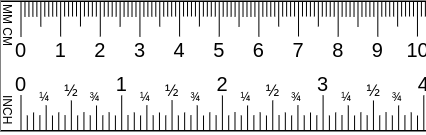
\includegraphics[width=4.1875in]{images/ruler-4-1875in}

\subsection{Significant Digit Rules}
\begin{enumerate}
    \item All non-zero digits are significant.
    \item Any zero digits between significant digits are significant.
    \item A trailing zero is significant only if it appears to the right of the decimal point.
\end{enumerate}
Example: How many significant digits are in each of the following?\newline
\begin{enumerate*}[label=\ \ (\alph*)]
    \item 1
    \item 10
    \item 1.0
    \item 10.0
    \item 0.000312
    \item 0.00300
\end{enumerate*}
\subsection{Addition with Significant Digits}
\begin{enumerate}
    \item Count the number of significant digits to the right of the decimal place in each of the numbers you are adding. This is the number of significant digits that your answer can have to the right of the decimal place.
    \item Add as normal.
    \item Round the sum to the correct number of significant digits.
\end{enumerate}
\subsection{Multiplication with Significant Digits}
\begin{enumerate}
    \item Count the number of significant digits in each number you are multiplying. This is the number of significant digits that can be in your answer.
    \item Multiply as normal.
    \item Round the product to the correct number of significant digits.
\end{enumerate}
Examples: \newline 
\begin{enumerate*}[label=\ \ (\alph*)]
    \item $10\mathrm{in} + 11\mathrm{in} = ?$
    \item $1\mathrm{mm} + 2.0\mathrm{mm} = ?$ 
    \item $1.125\mathrm{kg} + 0.1\mathrm{kg} = ?$
    \item $1.5\mathrm{in} \times 2.125\mathrm{in} = ?$ \newline
    \item $10.0\mathrm{mm} \times 2\mathrm{mm} = ?$
    \item Compute the Perimeter of your student ID.\newline
    \item Compute the area of your student ID.
\end{enumerate*}

\subsection{Siginificant Digits and Scientific Notation}
When using scientific notation, only write significant digits.

\subsection{When to Use Significant Digits}
Significant digit considerations only apply to values observed via measurement.  They do not apply to counting, abstract numbers, or theoretical values!


\end{document}
